% Clase 03 -- Ciclo de vida de los datos (Parte I): creacion/captura y
% transmision/almacenamiento.
% COMPILA desde esta carpeta (para que ../../tema/ resuelva), DOS pasadas:
%   pdflatex -shell-escape -interaction=nonstopmode slides.tex
%   pdflatex -shell-escape -interaction=nonstopmode slides.tex
% Solo caracteres ASCII (acentos con comandos LaTeX: \'a \~n \c{c}).
\documentclass[aspectratio=169]{beamer}
% El tema ya carga inputenc, fontenc y babel (spanish si esta instalado).
% molina-tema.tex
% Tema Beamer institucional ITJMM / Tecnologico Superior de Jalisco.
% Se carga con % molina-tema.tex
% Tema Beamer institucional ITJMM / Tecnologico Superior de Jalisco.
% Se carga con % molina-tema.tex
% Tema Beamer institucional ITJMM / Tecnologico Superior de Jalisco.
% Se carga con \input{../../tema/molina-tema.tex} desde slides.tex,
% que vive en clases/XX-tema/. COMPILAR SIEMPRE desde la carpeta de la
% clase para que las rutas relativas (../../tema/) resuelvan.
%
% Provee:
%   - Paleta institucional (molTeal, molNaranja, molAmarillo, molMorado).
%   - Franja vectorial de colores (\molinaBanner) en portada y separadores.
%   - Ambos logos (\molinaLogos) en portada y separadores.
%   - Slides de contenido limpias: titulo con regla teal + footline con
%     logo pequeno, titulo corto y numero de slide.
% Solo caracteres ASCII.

% Codificacion e idioma. Spanish de babel solo si esta instalado
% (texlive-lang-spanish); si no, cae a english para no romper el build.
\usepackage[utf8]{inputenc}
\usepackage[T1]{fontenc}
\IfFileExists{spanish.ldf}%
  {\usepackage[spanish]{babel}}%
  {\usepackage[english]{babel}}

\usepackage{tikz}
\usetikzlibrary{calc}
\usepackage{listings}

% --- Paleta (muestreada del master institucional) -----------------------
\definecolor{molTeal}{HTML}{0094A2}
\definecolor{molTealLt}{HTML}{00B0B5}
\definecolor{molNaranja}{HTML}{FE730C}
\definecolor{molRojo}{HTML}{FF5A0C}
\definecolor{molAmarillo}{HTML}{FEB200}
\definecolor{molMorado}{HTML}{532587}
\definecolor{molOro}{HTML}{B8860B}
\definecolor{molAzul}{HTML}{1F4E9B}

% --- Donde buscar logos y figuras ---------------------------------------
\graphicspath{{../../tema/}{figuras/}{datos/}}

% --- Colores de elementos Beamer ----------------------------------------
\setbeamercolor{structure}{fg=molTeal}
\setbeamercolor{frametitle}{fg=molTeal}
\setbeamercolor{title}{fg=molMorado}
\setbeamercolor{itemize item}{fg=molNaranja}
\setbeamercolor{itemize subitem}{fg=molTeal}
\setbeamercolor{block title}{bg=molTeal,fg=white}
\setbeamercolor{block body}{bg=molTeal!8,fg=black}
\setbeamertemplate{itemize items}[circle]
\setbeamertemplate{navigation symbols}{}

% --- Franja superior vectorial (formas angulares) -----------------------
% Anclada a las esquinas de la pagina; no depende del ancho exacto.
\newcommand{\molinaBanner}{%
  \begin{tikzpicture}[remember picture,overlay]
    \coordinate (O) at (current page.north west);
    \coordinate (E) at (current page.north east);
    % Bloque teal principal (izquierda)
    \fill[molTeal]    ($(O)+(0,0)$) -- ($(O)+(3.7,0)$) -- ($(O)+(3.1,-0.55)$) -- ($(O)+(0,-0.55)$) -- cycle;
    % Acento teal claro
    \fill[molTealLt]  ($(O)+(3.7,0)$) -- ($(O)+(4.5,0)$) -- ($(O)+(3.9,-0.55)$) -- ($(O)+(3.1,-0.55)$) -- cycle;
    % Muesca morada bajo el teal
    \fill[molMorado]  ($(O)+(0,-0.55)$) -- ($(O)+(0.75,-0.55)$) -- ($(O)+(0,-1.05)$) -- cycle;
    % Bloque naranja (centro-derecha)
    \fill[molNaranja] ($(E)+(-4.5,0)$) -- ($(E)+(-7.3,0)$) -- ($(E)+(-7.9,-0.55)$) -- ($(E)+(-5.1,-0.55)$) -- cycle;
    % Bloque rojo-naranja
    \fill[molRojo]    ($(E)+(-2.9,0)$) -- ($(E)+(-4.5,0)$) -- ($(E)+(-5.1,-0.55)$) -- ($(E)+(-3.5,-0.55)$) -- cycle;
    % Bloque amarillo (derecha)
    \fill[molAmarillo]($(E)+(0,0)$) -- ($(E)+(-2.9,0)$) -- ($(E)+(-3.5,-0.55)$) -- ($(E)+(0,-0.55)$) -- cycle;
  \end{tikzpicture}%
}

% --- Logos institucionales en el pie ------------------------------------
\newcommand{\molinaLogos}{%
  \begin{tikzpicture}[remember picture,overlay]
    \node[anchor=south west, inner sep=0pt]
      at ($(current page.south west)+(0.7cm,0.45cm)$)
      {
\includegraphics[height=1.05cm]{logo_mario_molina}};
    \node[anchor=south east, inner sep=0pt]
      at ($(current page.south east)+(-0.7cm,0.55cm)$)
      {
\includegraphics[height=0.85cm]{logo_TSJ}};
  \end{tikzpicture}%
}

% --- Portada -------------------------------------------------------------
% Usar dentro de \begin{frame}[plain]\titlepage\end{frame}
\setbeamertemplate{title page}{%
  \molinaBanner%
  \vfill
  \begin{center}
    {\usebeamercolor[fg]{title}\Large\bfseries\inserttitle\par}
    \vspace{0.4em}
    {\color{molTeal}\large\insertsubtitle\par}
    \vspace{1.6em}
    {\small\insertauthor\par}
    {\scriptsize\insertdate\par}
  \end{center}
  \vfill\vspace{1.0cm}%
  \molinaLogos%
}

% --- Separador de seccion -----------------------------------------------
\setbeamertemplate{section page}{%
  \molinaBanner%
  \vfill
  \begin{center}
    {\color{molTeal}\footnotesize SECCION\par}
    \vspace{0.3em}
    {\color{molMorado}\Large\bfseries\insertsectionhead\par}
  \end{center}
  \vfill\vspace{1.0cm}%
  \molinaLogos%
}
\AtBeginSection[]{%
  \begin{frame}[plain]\sectionpage\end{frame}%
}

% --- Frame de contenido: titulo con regla teal --------------------------
\setbeamertemplate{headline}{}
\setbeamertemplate{frametitle}{%
  \vspace*{0.4em}\hspace*{0.2em}%
  {\usebeamercolor[fg]{frametitle}\bfseries\insertframetitle}\par
  \vspace*{0.12em}\hspace*{0.2em}%
  {\color{molTeal}\rule{0.985\paperwidth}{1.2pt}}%
}

% --- Pie de slides de contenido -----------------------------------------
\setbeamertemplate{footline}{%
  \leavevmode%
  \hbox{%
    \begin{beamercolorbox}[wd=.22\paperwidth,ht=2.6ex,dp=1.1ex,leftskip=.4em]{}%
      \raisebox{-0.2ex}{
\includegraphics[height=1.7ex]{logo_mario_molina}}%
    \end{beamercolorbox}%
    \begin{beamercolorbox}[wd=.56\paperwidth,ht=2.6ex,dp=1.1ex,center]{}%
      {\scriptsize\color{molTeal}\insertshorttitle}%
    \end{beamercolorbox}%
    \begin{beamercolorbox}[wd=.22\paperwidth,ht=2.6ex,dp=1.1ex,rightskip=.4em]{}%
      \hfill{\scriptsize\color{molTeal}\insertframenumber}%
    \end{beamercolorbox}%
  }\vskip2pt%
}

% --- Estilo para bloques de codigo (listings) ---------------------------
\lstset{
  basicstyle=\ttfamily\small,
  keywordstyle=\color{molMorado}\bfseries,
  commentstyle=\color{molTeal}\itshape,
  stringstyle=\color{molNaranja},
  numberstyle=\tiny\color{gray},
  frame=single,
  rulecolor=\color{molTeal},
  backgroundcolor=\color{molTeal!5},
  breaklines=true,
  showstringspaces=false,
  tabsize=4,
  language=Python
}
 desde slides.tex,
% que vive en clases/XX-tema/. COMPILAR SIEMPRE desde la carpeta de la
% clase para que las rutas relativas (../../tema/) resuelvan.
%
% Provee:
%   - Paleta institucional (molTeal, molNaranja, molAmarillo, molMorado).
%   - Franja vectorial de colores (\molinaBanner) en portada y separadores.
%   - Ambos logos (\molinaLogos) en portada y separadores.
%   - Slides de contenido limpias: titulo con regla teal + footline con
%     logo pequeno, titulo corto y numero de slide.
% Solo caracteres ASCII.

% Codificacion e idioma. Spanish de babel solo si esta instalado
% (texlive-lang-spanish); si no, cae a english para no romper el build.
\usepackage[utf8]{inputenc}
\usepackage[T1]{fontenc}
\IfFileExists{spanish.ldf}%
  {\usepackage[spanish]{babel}}%
  {\usepackage[english]{babel}}

\usepackage{tikz}
\usetikzlibrary{calc}
\usepackage{listings}

% --- Paleta (muestreada del master institucional) -----------------------
\definecolor{molTeal}{HTML}{0094A2}
\definecolor{molTealLt}{HTML}{00B0B5}
\definecolor{molNaranja}{HTML}{FE730C}
\definecolor{molRojo}{HTML}{FF5A0C}
\definecolor{molAmarillo}{HTML}{FEB200}
\definecolor{molMorado}{HTML}{532587}
\definecolor{molOro}{HTML}{B8860B}
\definecolor{molAzul}{HTML}{1F4E9B}

% --- Donde buscar logos y figuras ---------------------------------------
\graphicspath{{../../tema/}{figuras/}{datos/}}

% --- Colores de elementos Beamer ----------------------------------------
\setbeamercolor{structure}{fg=molTeal}
\setbeamercolor{frametitle}{fg=molTeal}
\setbeamercolor{title}{fg=molMorado}
\setbeamercolor{itemize item}{fg=molNaranja}
\setbeamercolor{itemize subitem}{fg=molTeal}
\setbeamercolor{block title}{bg=molTeal,fg=white}
\setbeamercolor{block body}{bg=molTeal!8,fg=black}
\setbeamertemplate{itemize items}[circle]
\setbeamertemplate{navigation symbols}{}

% --- Franja superior vectorial (formas angulares) -----------------------
% Anclada a las esquinas de la pagina; no depende del ancho exacto.
\newcommand{\molinaBanner}{%
  \begin{tikzpicture}[remember picture,overlay]
    \coordinate (O) at (current page.north west);
    \coordinate (E) at (current page.north east);
    % Bloque teal principal (izquierda)
    \fill[molTeal]    ($(O)+(0,0)$) -- ($(O)+(3.7,0)$) -- ($(O)+(3.1,-0.55)$) -- ($(O)+(0,-0.55)$) -- cycle;
    % Acento teal claro
    \fill[molTealLt]  ($(O)+(3.7,0)$) -- ($(O)+(4.5,0)$) -- ($(O)+(3.9,-0.55)$) -- ($(O)+(3.1,-0.55)$) -- cycle;
    % Muesca morada bajo el teal
    \fill[molMorado]  ($(O)+(0,-0.55)$) -- ($(O)+(0.75,-0.55)$) -- ($(O)+(0,-1.05)$) -- cycle;
    % Bloque naranja (centro-derecha)
    \fill[molNaranja] ($(E)+(-4.5,0)$) -- ($(E)+(-7.3,0)$) -- ($(E)+(-7.9,-0.55)$) -- ($(E)+(-5.1,-0.55)$) -- cycle;
    % Bloque rojo-naranja
    \fill[molRojo]    ($(E)+(-2.9,0)$) -- ($(E)+(-4.5,0)$) -- ($(E)+(-5.1,-0.55)$) -- ($(E)+(-3.5,-0.55)$) -- cycle;
    % Bloque amarillo (derecha)
    \fill[molAmarillo]($(E)+(0,0)$) -- ($(E)+(-2.9,0)$) -- ($(E)+(-3.5,-0.55)$) -- ($(E)+(0,-0.55)$) -- cycle;
  \end{tikzpicture}%
}

% --- Logos institucionales en el pie ------------------------------------
\newcommand{\molinaLogos}{%
  \begin{tikzpicture}[remember picture,overlay]
    \node[anchor=south west, inner sep=0pt]
      at ($(current page.south west)+(0.7cm,0.45cm)$)
      {
\includegraphics[height=1.05cm]{logo_mario_molina}};
    \node[anchor=south east, inner sep=0pt]
      at ($(current page.south east)+(-0.7cm,0.55cm)$)
      {
\includegraphics[height=0.85cm]{logo_TSJ}};
  \end{tikzpicture}%
}

% --- Portada -------------------------------------------------------------
% Usar dentro de \begin{frame}[plain]\titlepage\end{frame}
\setbeamertemplate{title page}{%
  \molinaBanner%
  \vfill
  \begin{center}
    {\usebeamercolor[fg]{title}\Large\bfseries\inserttitle\par}
    \vspace{0.4em}
    {\color{molTeal}\large\insertsubtitle\par}
    \vspace{1.6em}
    {\small\insertauthor\par}
    {\scriptsize\insertdate\par}
  \end{center}
  \vfill\vspace{1.0cm}%
  \molinaLogos%
}

% --- Separador de seccion -----------------------------------------------
\setbeamertemplate{section page}{%
  \molinaBanner%
  \vfill
  \begin{center}
    {\color{molTeal}\footnotesize SECCION\par}
    \vspace{0.3em}
    {\color{molMorado}\Large\bfseries\insertsectionhead\par}
  \end{center}
  \vfill\vspace{1.0cm}%
  \molinaLogos%
}
\AtBeginSection[]{%
  \begin{frame}[plain]\sectionpage\end{frame}%
}

% --- Frame de contenido: titulo con regla teal --------------------------
\setbeamertemplate{headline}{}
\setbeamertemplate{frametitle}{%
  \vspace*{0.4em}\hspace*{0.2em}%
  {\usebeamercolor[fg]{frametitle}\bfseries\insertframetitle}\par
  \vspace*{0.12em}\hspace*{0.2em}%
  {\color{molTeal}\rule{0.985\paperwidth}{1.2pt}}%
}

% --- Pie de slides de contenido -----------------------------------------
\setbeamertemplate{footline}{%
  \leavevmode%
  \hbox{%
    \begin{beamercolorbox}[wd=.22\paperwidth,ht=2.6ex,dp=1.1ex,leftskip=.4em]{}%
      \raisebox{-0.2ex}{
\includegraphics[height=1.7ex]{logo_mario_molina}}%
    \end{beamercolorbox}%
    \begin{beamercolorbox}[wd=.56\paperwidth,ht=2.6ex,dp=1.1ex,center]{}%
      {\scriptsize\color{molTeal}\insertshorttitle}%
    \end{beamercolorbox}%
    \begin{beamercolorbox}[wd=.22\paperwidth,ht=2.6ex,dp=1.1ex,rightskip=.4em]{}%
      \hfill{\scriptsize\color{molTeal}\insertframenumber}%
    \end{beamercolorbox}%
  }\vskip2pt%
}

% --- Estilo para bloques de codigo (listings) ---------------------------
\lstset{
  basicstyle=\ttfamily\small,
  keywordstyle=\color{molMorado}\bfseries,
  commentstyle=\color{molTeal}\itshape,
  stringstyle=\color{molNaranja},
  numberstyle=\tiny\color{gray},
  frame=single,
  rulecolor=\color{molTeal},
  backgroundcolor=\color{molTeal!5},
  breaklines=true,
  showstringspaces=false,
  tabsize=4,
  language=Python
}
 desde slides.tex,
% que vive en clases/XX-tema/. COMPILAR SIEMPRE desde la carpeta de la
% clase para que las rutas relativas (../../tema/) resuelvan.
%
% Provee:
%   - Paleta institucional (molTeal, molNaranja, molAmarillo, molMorado).
%   - Franja vectorial de colores (\molinaBanner) en portada y separadores.
%   - Ambos logos (\molinaLogos) en portada y separadores.
%   - Slides de contenido limpias: titulo con regla teal + footline con
%     logo pequeno, titulo corto y numero de slide.
% Solo caracteres ASCII.

% Codificacion e idioma. Spanish de babel solo si esta instalado
% (texlive-lang-spanish); si no, cae a english para no romper el build.
\usepackage[utf8]{inputenc}
\usepackage[T1]{fontenc}
\IfFileExists{spanish.ldf}%
  {\usepackage[spanish]{babel}}%
  {\usepackage[english]{babel}}

\usepackage{tikz}
\usetikzlibrary{calc}
\usepackage{listings}

% --- Paleta (muestreada del master institucional) -----------------------
\definecolor{molTeal}{HTML}{0094A2}
\definecolor{molTealLt}{HTML}{00B0B5}
\definecolor{molNaranja}{HTML}{FE730C}
\definecolor{molRojo}{HTML}{FF5A0C}
\definecolor{molAmarillo}{HTML}{FEB200}
\definecolor{molMorado}{HTML}{532587}
\definecolor{molOro}{HTML}{B8860B}
\definecolor{molAzul}{HTML}{1F4E9B}

% --- Donde buscar logos y figuras ---------------------------------------
\graphicspath{{../../tema/}{figuras/}{datos/}}

% --- Colores de elementos Beamer ----------------------------------------
\setbeamercolor{structure}{fg=molTeal}
\setbeamercolor{frametitle}{fg=molTeal}
\setbeamercolor{title}{fg=molMorado}
\setbeamercolor{itemize item}{fg=molNaranja}
\setbeamercolor{itemize subitem}{fg=molTeal}
\setbeamercolor{block title}{bg=molTeal,fg=white}
\setbeamercolor{block body}{bg=molTeal!8,fg=black}
\setbeamertemplate{itemize items}[circle]
\setbeamertemplate{navigation symbols}{}

% --- Franja superior vectorial (formas angulares) -----------------------
% Anclada a las esquinas de la pagina; no depende del ancho exacto.
\newcommand{\molinaBanner}{%
  \begin{tikzpicture}[remember picture,overlay]
    \coordinate (O) at (current page.north west);
    \coordinate (E) at (current page.north east);
    % Bloque teal principal (izquierda)
    \fill[molTeal]    ($(O)+(0,0)$) -- ($(O)+(3.7,0)$) -- ($(O)+(3.1,-0.55)$) -- ($(O)+(0,-0.55)$) -- cycle;
    % Acento teal claro
    \fill[molTealLt]  ($(O)+(3.7,0)$) -- ($(O)+(4.5,0)$) -- ($(O)+(3.9,-0.55)$) -- ($(O)+(3.1,-0.55)$) -- cycle;
    % Muesca morada bajo el teal
    \fill[molMorado]  ($(O)+(0,-0.55)$) -- ($(O)+(0.75,-0.55)$) -- ($(O)+(0,-1.05)$) -- cycle;
    % Bloque naranja (centro-derecha)
    \fill[molNaranja] ($(E)+(-4.5,0)$) -- ($(E)+(-7.3,0)$) -- ($(E)+(-7.9,-0.55)$) -- ($(E)+(-5.1,-0.55)$) -- cycle;
    % Bloque rojo-naranja
    \fill[molRojo]    ($(E)+(-2.9,0)$) -- ($(E)+(-4.5,0)$) -- ($(E)+(-5.1,-0.55)$) -- ($(E)+(-3.5,-0.55)$) -- cycle;
    % Bloque amarillo (derecha)
    \fill[molAmarillo]($(E)+(0,0)$) -- ($(E)+(-2.9,0)$) -- ($(E)+(-3.5,-0.55)$) -- ($(E)+(0,-0.55)$) -- cycle;
  \end{tikzpicture}%
}

% --- Logos institucionales en el pie ------------------------------------
\newcommand{\molinaLogos}{%
  \begin{tikzpicture}[remember picture,overlay]
    \node[anchor=south west, inner sep=0pt]
      at ($(current page.south west)+(0.7cm,0.45cm)$)
      {
\includegraphics[height=1.05cm]{logo_mario_molina}};
    \node[anchor=south east, inner sep=0pt]
      at ($(current page.south east)+(-0.7cm,0.55cm)$)
      {
\includegraphics[height=0.85cm]{logo_TSJ}};
  \end{tikzpicture}%
}

% --- Portada -------------------------------------------------------------
% Usar dentro de \begin{frame}[plain]\titlepage\end{frame}
\setbeamertemplate{title page}{%
  \molinaBanner%
  \vfill
  \begin{center}
    {\usebeamercolor[fg]{title}\Large\bfseries\inserttitle\par}
    \vspace{0.4em}
    {\color{molTeal}\large\insertsubtitle\par}
    \vspace{1.6em}
    {\small\insertauthor\par}
    {\scriptsize\insertdate\par}
  \end{center}
  \vfill\vspace{1.0cm}%
  \molinaLogos%
}

% --- Separador de seccion -----------------------------------------------
\setbeamertemplate{section page}{%
  \molinaBanner%
  \vfill
  \begin{center}
    {\color{molTeal}\footnotesize SECCION\par}
    \vspace{0.3em}
    {\color{molMorado}\Large\bfseries\insertsectionhead\par}
  \end{center}
  \vfill\vspace{1.0cm}%
  \molinaLogos%
}
\AtBeginSection[]{%
  \begin{frame}[plain]\sectionpage\end{frame}%
}

% --- Frame de contenido: titulo con regla teal --------------------------
\setbeamertemplate{headline}{}
\setbeamertemplate{frametitle}{%
  \vspace*{0.4em}\hspace*{0.2em}%
  {\usebeamercolor[fg]{frametitle}\bfseries\insertframetitle}\par
  \vspace*{0.12em}\hspace*{0.2em}%
  {\color{molTeal}\rule{0.985\paperwidth}{1.2pt}}%
}

% --- Pie de slides de contenido -----------------------------------------
\setbeamertemplate{footline}{%
  \leavevmode%
  \hbox{%
    \begin{beamercolorbox}[wd=.22\paperwidth,ht=2.6ex,dp=1.1ex,leftskip=.4em]{}%
      \raisebox{-0.2ex}{
\includegraphics[height=1.7ex]{logo_mario_molina}}%
    \end{beamercolorbox}%
    \begin{beamercolorbox}[wd=.56\paperwidth,ht=2.6ex,dp=1.1ex,center]{}%
      {\scriptsize\color{molTeal}\insertshorttitle}%
    \end{beamercolorbox}%
    \begin{beamercolorbox}[wd=.22\paperwidth,ht=2.6ex,dp=1.1ex,rightskip=.4em]{}%
      \hfill{\scriptsize\color{molTeal}\insertframenumber}%
    \end{beamercolorbox}%
  }\vskip2pt%
}

% --- Estilo para bloques de codigo (listings) ---------------------------
\lstset{
  basicstyle=\ttfamily\small,
  keywordstyle=\color{molMorado}\bfseries,
  commentstyle=\color{molTeal}\itshape,
  stringstyle=\color{molNaranja},
  numberstyle=\tiny\color{gray},
  frame=single,
  rulecolor=\color{molTeal},
  backgroundcolor=\color{molTeal!5},
  breaklines=true,
  showstringspaces=false,
  tabsize=4,
  language=Python
}


\usetikzlibrary{positioning,arrows.meta,shapes.geometric,fit,backgrounds}

\title{Clase 03 -- Ciclo de vida de los datos (Parte I)}
\subtitle{Creaci\'on y captura; Transmisi\'on y almacenamiento}
\author{Instituto Tecnol\'ogico Jos\'e Mario Molina Pasquel y Henr\'iquez}
\date{\today}

\begin{document}

% ----------------------------------------------------------------------
% Portada
\begin{frame}[plain]
  \titlepage
\end{frame}

% ----------------------------------------------------------------------
% Agenda
\begin{frame}{Agenda}
  \tableofcontents
\end{frame}

% ======================================================================
\section{El ciclo de vida de los datos}

\begin{frame}{El ciclo de vida de los datos}
  \begin{columns}[c]
    \column{0.6\textwidth}
      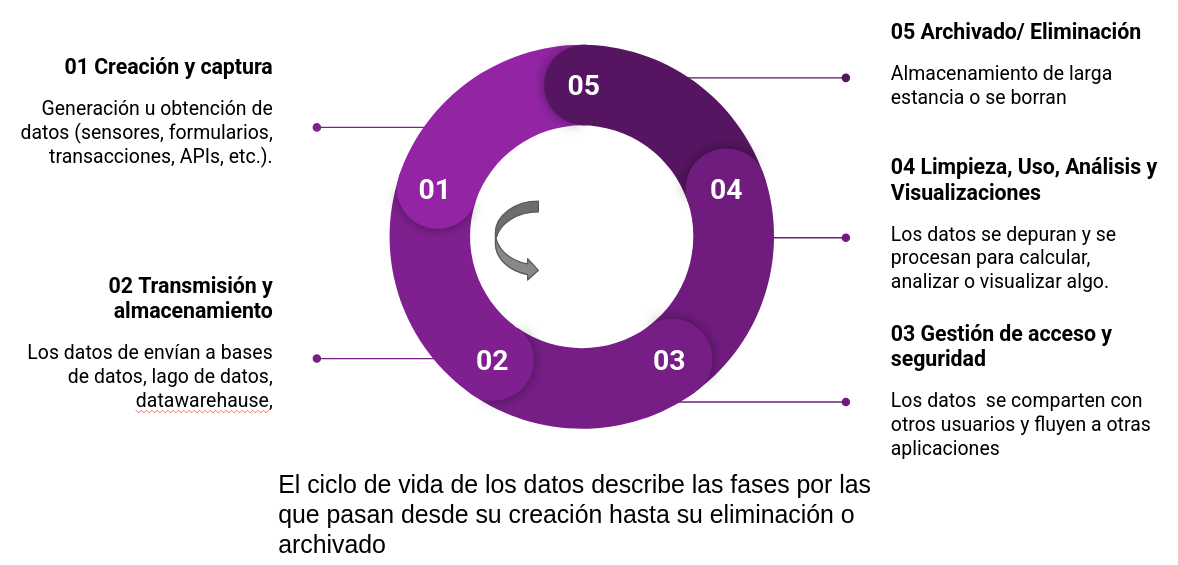
\includegraphics[width=\linewidth]{_fuentes/imagenes/ciclo_vida_completo}
    \column{0.4\textwidth}
      Describe las fases por las que pasan los datos desde su creaci\'on hasta
      su eliminaci\'on o archivado.
      \begin{block}{En esta clase (Parte I)}
        Vemos a detalle las etapas \textbf{01 Creaci\'on y captura} y
        \textbf{02 Transmisi\'on y almacenamiento}.
      \end{block}
  \end{columns}
\end{frame}

% ======================================================================
\section{Etapa 01: Creaci\'on y captura}

\begin{frame}{Creaci\'on y captura: definici\'on y errores}
  \begin{columns}[t]
    \column{0.5\textwidth}
      \textbf{Definici\'on}\\[2pt]
      Generaci\'on u obtenci\'on de datos: sensores, formularios,
      transacciones, APIs, etc.
    \column{0.5\textwidth}
      \begin{block}{Posibles errores}
        \begin{itemize}
          \item Datos incompletos (campos vac\'ios).
          \item Datos duplicados.
          \item Errores de formato (fecha como texto:
                ``12/31/2024'' vs ``31-12-2024'').
          \item Sesgo en la recolecci\'on (muestras no representativas).
          \item Codificaci\'on distinta (UTF-8).
        \end{itemize}
      \end{block}
  \end{columns}
\end{frame}

\begin{frame}[fragile]{?`C\'omo se capturan los datos?}
  \begin{center}
  \begin{tikzpicture}[
      font=\scriptsize,
      root/.style={rounded corners, draw=molTeal, very thick, fill=molTeal!12,
                   font=\small\bfseries, minimum width=2.6cm, minimum height=0.7cm},
      m/.style={rounded corners, draw=#1, very thick, fill=#1!15,
                font=\scriptsize\bfseries, align=center, minimum width=2.0cm,
                minimum height=0.75cm},
      every node/.style={align=center}]
    \node[root] (r) at (5.5,3.0) {Captura de datos};
    \node[m=molMorado]  (cen) at (0.5,1.5) {Censo};
    \node[m=molMorado]  (enc) at (2.7,1.5) {Encuesta};
    \node[m=molMorado]  (son) at (4.9,1.5) {Sondeo};
    \node[m=molNaranja] (adm) at (7.1,1.5) {Datos\\admin.};
    \node[m=molNaranja] (sen) at (9.3,1.5) {Sensores};
    \node[m=molAzul]    (cam) at (2.7,0.1) {Levant.\\en campo};
    \node[m=molAzul]    (min) at (4.9,0.1) {Miner\'ia\\de datos};
    \node[m=molAzul]    (big) at (7.1,0.1) {Big data};
    \foreach \n in {cen,enc,son,adm,sen} {\draw[molTeal,thick] (r) -- (\n);}
    \foreach \n in {cam,min,big} {\draw[molTeal,thick] (r) -- (\n);}
  \end{tikzpicture}
  \end{center}
  Cada m\'etodo tiene un costo, una cobertura y un nivel de error distintos.
\end{frame}

\begin{frame}{Censo}
  \begin{columns}[t]
    \column{0.52\textwidth}
      Recopilaci\'on \textbf{sistem\'atica y exhaustiva} de datos de
      \textbf{toda la poblaci\'on} de inter\'es (no solo una muestra).
      \begin{itemize}
        \item Busca datos completos, no inferidos.
        \item La metodolog\'ia determina el nivel de confianza y error.
      \end{itemize}
    \column{0.48\textwidth}
      \begin{block}{Retos}
        \begin{itemize}
          \item Alto costo (recursos, log\'istica, tiempo).
          \item Cobertura completa (zonas remotas).
          \item Actualizaci\'on (se vuelve obsoleto).
          \item Participaci\'on (resistencia a responder).
        \end{itemize}
      \end{block}
  \end{columns}
\end{frame}

\begin{frame}{El censo es un proceso mayor}
  \begin{columns}[t]
    \column{0.5\textwidth}
      \textbf{Etapas tipicas}
      \begin{enumerate}
        \item Objetivos y alcance.
        \item Marco legal y financiamiento.
        \item Dise\~no metodol\'ogico.
        \item Prueba piloto.
        \item Recolecci\'on y monitoreo.
        \item Procesamiento y validaci\'on.
        \item Difusi\'on y evaluaci\'on.
      \end{enumerate}
    \column{0.5\textwidth}
      \begin{block}{Tipos de censo}
        \begin{itemize}
          \item Poblaci\'on y vivienda (cada 10 anios).
          \item Econ\'omicos (cada 5 anios).
          \item Agropecuario (cada 10 anios).
          \item De gobierno (anual / bienal).
        \end{itemize}
      \end{block}
      \footnotesize En M\'exico: el INEGI (creado en 1983) levanta el Censo de
      Poblaci\'on y Vivienda; en 2020 conto 126 millones de personas.
  \end{columns}
\end{frame}

\begin{frame}{Encuesta}
  \begin{columns}[t]
    \column{0.55\textwidth}
      Recolecci\'on mediante cuestionarios aplicados a una \textbf{muestra
      representativa} para \emph{inferir} sobre toda la poblaci\'on.
      \begin{itemize}
        \item Muestra aleatoria; se buscan tendencias generales.
        \item El margen de error es aceptable y conocido.
      \end{itemize}
      \begin{block}{Confianza del 95\%, error +/- 3\%}
        Si se repitiera el estudio 100 veces, en 95 los resultados caer\'ian
        dentro del margen. \textbf{No} garantiza exactitud: hay 95\% de
        probabilidad de estar cerca de lo real.
      \end{block}
    \column{0.45\textwidth}
      \begin{block}{Retos}
        \begin{itemize}
          \item Dise\~no del cuestionario (preguntas sesgadas).
          \item Tasa de respuesta (no respuesta).
          \item Sesgos (deseabilidad social).
          \item Costo en muestras grandes.
        \end{itemize}
      \end{block}
  \end{columns}
\end{frame}

\begin{frame}{Otros m\'etodos de captura}
  \begin{columns}[t]
    \column{0.5\textwidth}
      \begin{block}{Sondeo}
        R\'apido y \textbf{no exhaustivo}; visi\'on preliminar. M\'as errores y
        sesgos; resultados \textbf{no generalizables}.
      \end{block}
      \begin{block}{Datos administrativos}
        Recolectados para fines \textbf{no estad\'isticos} (salud, impuestos).
        Retos: calidad inconsistente y acceso restringido.
      \end{block}
    \column{0.5\textwidth}
      \begin{block}{Sensores}
        Medici\'on \textbf{directa o indirecta} y monitoreo continuo. Retos:
        costo y acceso (privacidad).
      \end{block}
      \begin{block}{Levantamiento en campo}
        Recolecci\'on \textbf{in situ} (observaci\'on, mediciones). Retos:
        accesibilidad, precisi\'on, clima, log\'istica.
      \end{block}
  \end{columns}
\end{frame}

\begin{frame}[fragile]{Miner\'ia de datos y Big Data: las 5 V}
  \begin{center}
  \begin{tikzpicture}[
      v/.style={rounded corners, draw=#1, very thick, fill=#1!15,
                minimum width=2.0cm, minimum height=1.3cm, align=center,
                font=\scriptsize\bfseries},
      every node/.style={align=center}]
    \node[v=molTeal]    (vo) at (0,0)    {Volumen\\[2pt]\mdseries cantidad};
    \node[v=molNaranja] (ve) at (2.3,0)  {Velocidad\\[2pt]\mdseries generaci\'on};
    \node[v=molAmarillo](va) at (4.6,0)  {Variedad\\[2pt]\mdseries diversidad};
    \node[v=molMorado]  (vc) at (6.9,0)  {Veracidad\\[2pt]\mdseries exactitud};
    \node[v=molAzul]    (vl) at (9.2,0)  {Valor\\[2pt]\mdseries utilidad};
  \end{tikzpicture}
  \end{center}
  \vspace{0.3em}
  \textbf{Big data}: colecciones enormes y diversas (estructuradas, semi y no
  estructuradas) que crecen y que los sistemas tradicionales no pueden
  almacenar/procesar. \textbf{Miner\'ia de datos}: analizar esos grandes
  vol\'umenes para hallar patrones.
  \vspace{0.2em}\\
  \footnotesize T\'ecnicas: MapReduce, c\'omputo paralelo y muestreo (sampling).
\end{frame}

\begin{frame}{Fuentes de datos abiertos}
  Muchos datos ya estan creados y disponibles para reutilizarse:
  \begin{columns}[t]
    \column{0.5\textwidth}
      \begin{itemize}
        \item \textbf{M\'exico}: datos.gob.mx, iiieg.gob.mx
        \item \textbf{EE.UU.}: Data.gov
        \item \textbf{Uni\'on Europea}: European Data Portal
        \item \textbf{Reino Unido}: data.gov.uk
      \end{itemize}
    \column{0.5\textwidth}
      \begin{itemize}
        \item \textbf{NASA}: Open Data Portal
        \item \textbf{NOAA / ESA}: clima e im\'agenes satelitales
        \item \textbf{Kaggle}, \textbf{DrivenData}: datasets
      \end{itemize}
  \end{columns}
  \vspace{0.4em}
  Antes de capturar datos nuevos, conviene revisar si ya existen.
\end{frame}

% ======================================================================
\section{Etapa 02: Transmisi\'on y almacenamiento}

\begin{frame}{Transmisi\'on y almacenamiento: definici\'on y errores}
  \begin{columns}[t]
    \column{0.46\textwidth}
      \textbf{Definici\'on}\\[2pt]
      Los datos se env\'ian y guardan en bases de datos, \emph{data lakes} o
      \emph{data warehouses} para su uso posterior.
    \column{0.54\textwidth}
      \begin{block}{Posibles errores}
        \begin{itemize}
          \item P\'erdida por fallos de hardware.
          \item Almacenamiento redundante / duplicidad.
          \item Estructura inadecuada (tablas mal normalizadas).
          \item Sin respaldo (regla 3-2-1) o respaldos no peri\'odicos.
          \item Corrupci\'on de datos; errores en el ETL.
          \item Formatos incompatibles.
        \end{itemize}
      \end{block}
  \end{columns}
\end{frame}

\begin{frame}[fragile]{Buena pr\'actica de respaldo: la regla 3-2-1}
  \begin{center}
  \begin{tikzpicture}[
      b/.style={rounded corners, draw=#1, very thick, fill=#1!12,
                minimum width=3.2cm, minimum height=2.0cm, align=center,
                font=\footnotesize},
      every node/.style={align=center}]
    \node[b=molTeal]    (a) at (0,0)   {{\Large\bfseries\color{molTeal} 3}\\[3pt]copias de\\ los datos};
    \node[b=molNaranja] (b) at (4.2,0) {{\Large\bfseries\color{molNaranja} 2}\\[3pt]tipos de\\ medios distintos};
    \node[b=molMorado]  (c) at (8.4,0) {{\Large\bfseries\color{molMorado} 1}\\[3pt]copia fuera\\ del sitio};
  \end{tikzpicture}
  \end{center}
  \vspace{0.3em}
  Mantener \textbf{tres} copias de los datos, en \textbf{dos} tipos de medios y
  con \textbf{una} copia fuera del sitio reduce el riesgo de perderlo todo.
\end{frame}

\begin{frame}[fragile]{ETL: Extract -- Transform -- Load}
  \begin{center}
  \begin{tikzpicture}[
      s/.style={rounded corners, draw=#1, very thick, fill=#1!12,
                minimum width=2.3cm, minimum height=1.0cm, align=center,
                font=\footnotesize\bfseries},
      every node/.style={align=center}]
    \node[s=gray]       (src) at (0,0)   {Fuentes};
    \node[s=molTeal]    (e)   at (2.9,0) {Extract\\\scriptsize\mdseries obtener};
    \node[s=molNaranja] (t)   at (5.8,0) {Transform\\\scriptsize\mdseries limpiar};
    \node[s=molMorado]  (l)   at (8.7,0) {Load\\\scriptsize\mdseries cargar};
    \node[s=molAzul]    (dst) at (11.4,0){Destino};
    \draw[-{Latex[length=2mm]},thick] (src)--(e);
    \draw[-{Latex[length=2mm]},thick] (e)--(t);
    \draw[-{Latex[length=2mm]},thick] (t)--(l);
    \draw[-{Latex[length=2mm]},thick] (l)--(dst);
  \end{tikzpicture}
  \end{center}
  \vspace{0.2em}
  El ETL mueve los datos desde las fuentes hacia el siguiente proceso (``el
  plomero de los datos''): \textbf{Extract} obtiene, \textbf{Transform} limpia y
  calcula, \textbf{Load} carga en el repositorio destino.
\end{frame}

\begin{frame}{?`D\'onde se guardan? Lake, Warehouse y Lakehouse}
  \begin{columns}[t]
    \column{0.5\textwidth}
      \begin{block}{Data Lake}
        Repositorio de datos \textbf{en bruto} (estructurados, semi y no
        estructurados), esquema flexible (\emph{schema-on-read}), escalable
        (Hadoop, AWS S3).
      \end{block}
    \column{0.5\textwidth}
      \begin{block}{Data Warehouse}
        Repositorio \textbf{centralizado} de datos estructurados y
        \textbf{procesados} (ETL), esquema fijo (\emph{schema-on-write}),
        orientado a consultas y reportes (Snowflake, BigQuery).
      \end{block}
  \end{columns}
  \vspace{0.3em}
  El \textbf{Data Lakehouse} combina ambos: la flexibilidad del lake con una capa
  de gobierno y metadatos para analitica y ML.
\end{frame}

\begin{frame}{Data Warehouse vs Data Lake}
  \small
  \begin{center}
  \begin{tabular}{p{2.4cm} p{4.0cm} p{4.0cm}}
    \textbf{Aspecto} & \textbf{Data Warehouse} & \textbf{Data Lake}\\[2pt]
    \hline
    Tipo de datos & Solo estructurados (SQL) & Cualquier tipo (JSON, im\'agenes, logs)\\[2pt]
    Procesamiento & Transformados antes (ETL) & En crudo (se procesan al leer)\\[2pt]
    Esquema & \emph{schema-on-write} & \emph{schema-on-read}\\[2pt]
    Usuarios & Analistas de BI & Cient\'ificos de datos / ingenieros\\[2pt]
    Herramientas & Snowflake, Redshift, BigQuery & Hadoop, AWS S3, Azure Data Lake\\
    \hline
  \end{tabular}
  \end{center}
\end{frame}

\begin{frame}[fragile]{La tuber\'ia de datos (data pipeline)}
  \begin{center}
  \begin{tikzpicture}[
      st/.style={rounded corners, draw=molTeal, very thick, fill=molTeal!12,
                 minimum width=1.8cm, minimum height=0.9cm, align=center,
                 font=\scriptsize\bfseries},
      every node/.style={align=center}]
    \node[st] (so) at (0,0)    {Source};
    \node[st] (in) at (2.1,0)  {Ingest};
    \node[st] (st) at (4.2,0)  {Store};
    \node[st] (tr) at (6.3,0)  {Transform};
    \node[st] (pu) at (8.4,0)  {Publish};
    \node[st] (co) at (10.5,0) {Consume};
    \foreach \a/\b in {so/in,in/st,st/tr,tr/pu,pu/co}
      {\draw[-{Latex[length=2mm]},thick] (\a)--(\b);}
    \node[draw=molMorado, very thick, rounded corners, fill=molMorado!8,
          minimum width=11.6cm, minimum height=0.55cm, font=\scriptsize,
          below=0.4cm of tr, xshift=0cm] (mg)
      {Management: metadatos, calidad, gobernanza, privacidad, protecci\'on};
  \end{tikzpicture}
  \end{center}
  \vspace{0.2em}
  Una arquitectura de datos encadena estas etapas; debajo, una capa transversal
  de gobierno vigila calidad, privacidad y seguridad.
\end{frame}

\begin{frame}{Orquestaci\'on de datos}
  \begin{columns}[c]
    \column{0.58\textwidth}
      Es el proceso de \textbf{extraer datos aislados} de m\'ultiples
      ubicaciones, combinarlos, organizarlos y ponerlos a disposici\'on del
      an\'alisis. Incluye aprovisionar recursos y \textbf{monitorear}.
      \vspace{0.4em}
      \begin{itemize}
        \item Automatiza pipelines ETL/ELT que corren solos y se reintentan.
        \item Disparadores: por horario, por evento o por dependencia.
      \end{itemize}
    \column{0.42\textwidth}
      \begin{block}{Herramientas}
        \begin{itemize}
          \item Apache Airflow
          \item Luigi (Spotify)
          \item Oozie, Azkaban
          \item Control-M, AutoSys
        \end{itemize}
      \end{block}
  \end{columns}
\end{frame}

\begin{frame}[fragile]{Apache Airflow}
  \begin{columns}[c]
    \column{0.46\textwidth}
      \begin{tikzpicture}[
          n/.style={circle, draw=molTeal, very thick, fill=molTeal!18,
                    font=\scriptsize\bfseries, minimum size=0.85cm},
          every node/.style={align=center}]
        \node[n] (a) at (0,0)     {extract};
        \node[n] (b) at (2.4,0.8) {clean};
        \node[n] (c) at (2.4,-0.8){validate};
        \node[n] (d) at (4.8,0)   {load};
        \draw[-{Latex[length=2mm]},molMorado,thick] (a)--(b);
        \draw[-{Latex[length=2mm]},molMorado,thick] (a)--(c);
        \draw[-{Latex[length=2mm]},molMorado,thick] (b)--(d);
        \draw[-{Latex[length=2mm]},molMorado,thick] (c)--(d);
      \end{tikzpicture}
      \\[4pt]
      \footnotesize Un \textbf{DAG}: tareas ordenadas sin ciclos.
    \column{0.54\textwidth}
      Plataforma open-source (en Python) para \textbf{orquestar workflows}.
      \begin{itemize}
        \item \textbf{DAG}: grafo ac\'iclico dirigido de tareas.
        \item \textbf{Operators}: bloques (PythonOperator, BashOperator).
        \item \textbf{Tasks}: instancias de un operator.
        \item \textbf{Scheduler}: ejecuta seg\'un dependencias.
        \item \textbf{Executor}: define c\'omo corren (Local, Celery).
      \end{itemize}
  \end{columns}
\end{frame}

\begin{frame}[fragile]{Un DAG minimo en Airflow}
\begin{lstlisting}[language=Python, basicstyle=\ttfamily\scriptsize]
from airflow import DAG
from airflow.operators.python import PythonOperator
import datetime as dt

with DAG("etl_diario", schedule="@daily",
         start_date=dt.datetime(2026, 1, 1)) as dag:

    extraer = PythonOperator(task_id="extraer", python_callable=extract)
    limpiar = PythonOperator(task_id="limpiar", python_callable=transform)
    cargar  = PythonOperator(task_id="cargar",  python_callable=load)

    extraer >> limpiar >> cargar    # define el orden
\end{lstlisting}
  El operador \texttt{>>} fija las dependencias: primero extraer, luego limpiar,
  luego cargar.
\end{frame}

% ======================================================================
\section{Resumen}

\begin{frame}{Takeaways}
  \begin{itemize}
    \item El \textbf{ciclo de vida} va de la creaci\'on al archivado; hoy vimos
          \textbf{captura} y \textbf{almacenamiento}.
    \item La \textbf{captura} tiene muchos m\'etodos (censo, encuesta, sondeo,
          sensores, big data); cada uno con su costo, cobertura y error.
    \item Una \textbf{encuesta} infiere de una muestra: confianza del 95\% no es
          exactitud, sino probabilidad de estar cerca.
    \item En \textbf{almacenamiento}, respaldar con la regla \textbf{3-2-1} y
          mover datos con \textbf{ETL}.
    \item \textbf{Data Lake} (crudo, flexible) vs \textbf{Data Warehouse}
          (estructurado, ETL); el \textbf{Lakehouse} combina ambos.
    \item La \textbf{orquestaci\'on} (Airflow y sus DAGs) automatiza y vigila los
          pipelines.
  \end{itemize}
\end{frame}

\begin{frame}[plain]
  \molinaBanner
  \vfill
  \begin{center}
    {\color{molMorado}\Large\bfseries Gracias}\\[0.4em]
    {\color{molTeal} Siguiente (Parte II): acceso y seguridad; limpieza,
     an\'alisis y visualizaci\'on}
  \end{center}
  \vfill\vspace{1.0cm}
  \molinaLogos
\end{frame}

\end{document}
